\documentclass{vilniustech-en}
\vilniustechsetup{
    university={Vilnius Gediminas technical university},
    faculty={Faculty of Fundamental Sciences},
    cathedral={Department of Information Systems},
    workTitle={Ethical Hacking Techniques},
    workType={Laboratory Work 1},
    workAuthorName={Aurimas Šakalys},
    workAuthorGroup={ITSfm-22},
    workRecipient={lecturer Leonardas Marozas}
}
\addbibresource{bibliography.bib}
\VTDocumentBegin


\section{Target}

The target we will be footprinting is \textit{NexusMods}. Their main domain is \textit{*.nexusmods.com}, and they are particapating in \textit{OpenBugBounty} (\textit{OBB}) program, \url{https://www.openbugbounty.org/bugbounty/tomrmason}.


\section{Goals}
We could peform both passive and active reconaisance, but the entry within \textit{OBB} states clearly, that any social-engineering attacks are disallowed. While gathering of social information would be possible, for practice purposes, we shall skip identification of individuals due to legal and moral reasons, but we shall look over some public data on the institution itself.

We will be performing the reconaisance with the goal of finding the information that would allow us to reduce the attack surface, and possibly identify IP ranges, controlled domains by \textit{NexusMods}.

For technical part we shall use local tools and \url{osintframework.com}

\section{Registrars, Names and IPs}

\subsection{\textit{whois}}

We use a local tool \textit{whois}, to gather some information about the registered entity (\autoref{fig:whois_initial}). We can see, that it is registered in Iceland (\autoref{fig:whois_later}) and it's name servers are within \textit{Cloudflare} services (\autoref{fig:whois_name_servers}).

\begin{figure}[H]
\begin{center}
    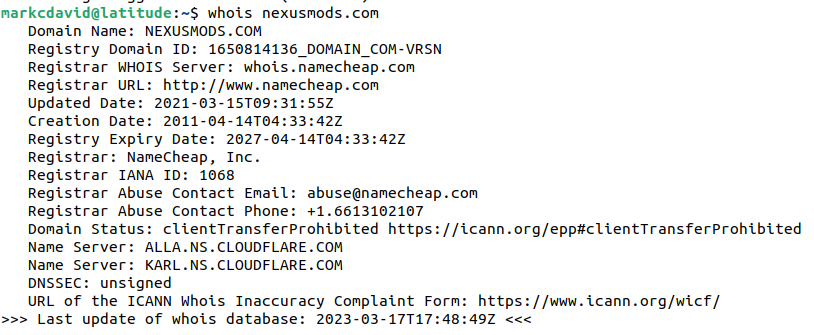
\includegraphics[width=16cm]{img/whois_initial.png}
    \caption{Initial results of the \textit{whois} command}
    \label{fig:whois_initial}
\end{center}
\end{figure}

\begin{figure}[H]
\begin{center}
    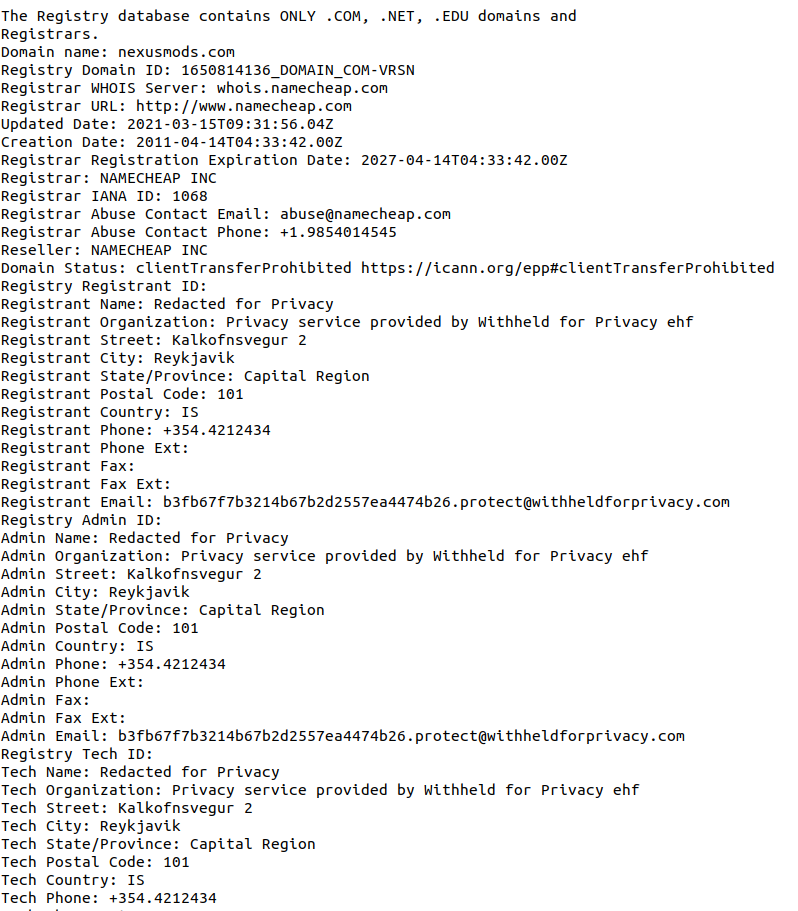
\includegraphics[width=16cm]{img/whois_later.png}
    \caption{Additional results of the \textit{whois} command}
    \label{fig:whois_later}
\end{center}
\end{figure}

\begin{figure}[H]
\begin{center}
    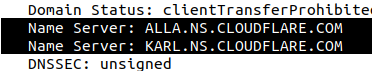
\includegraphics[width=16cm]{img/whois_name_servers.png}
    \caption{Nameserver information from \textit{whois} command}
    \label{fig:whois_name_servers}
\end{center}
\end{figure}

Given the experience with \textit{Cloudflare}, it could mean that we would have difficult time extracting DNS data for the institution.

We can see where in Reykjavik the address mentioned in whois records is located (\autoref{fig:open_street_map_reykiavik}). As the data is duplicated across registrant, admin and tech, it might indicate redaction due to priacy reasons.

\begin{figure}[H]
\begin{center}
    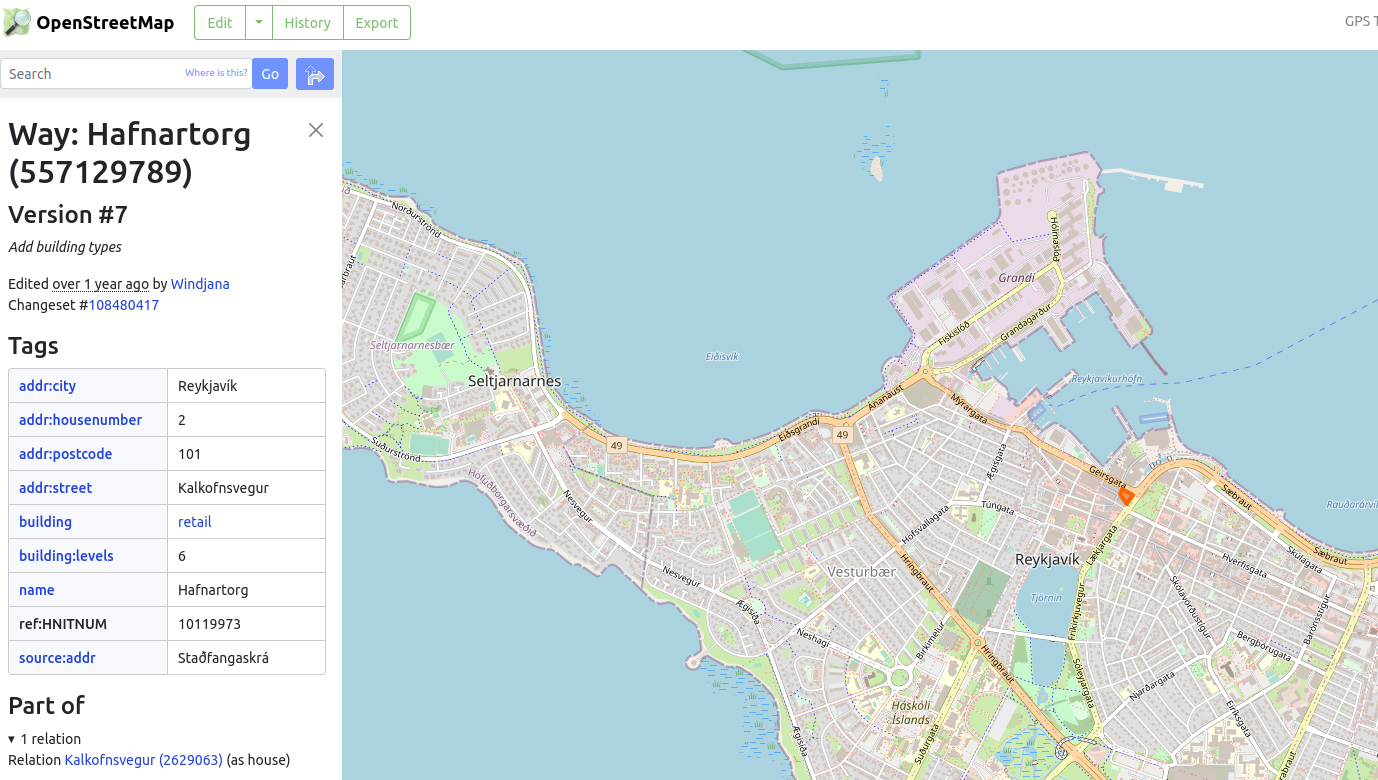
\includegraphics[width=16cm]{img/open_street_map_reykiavik.png}
    \caption{Location of the Reykjavik office in \textit{OpenStreetMap}}
    \label{fig:open_street_map_reykiavik}
\end{center}
\end{figure}

We can prove this to ourselves, simply by looking to the \textit{About Us} section of \textit{NexusMods} website, to see that they are actually based in the UK (\autoref{fig:nexusmods_about_us}). 

\begin{figure}[H]
\begin{center}
    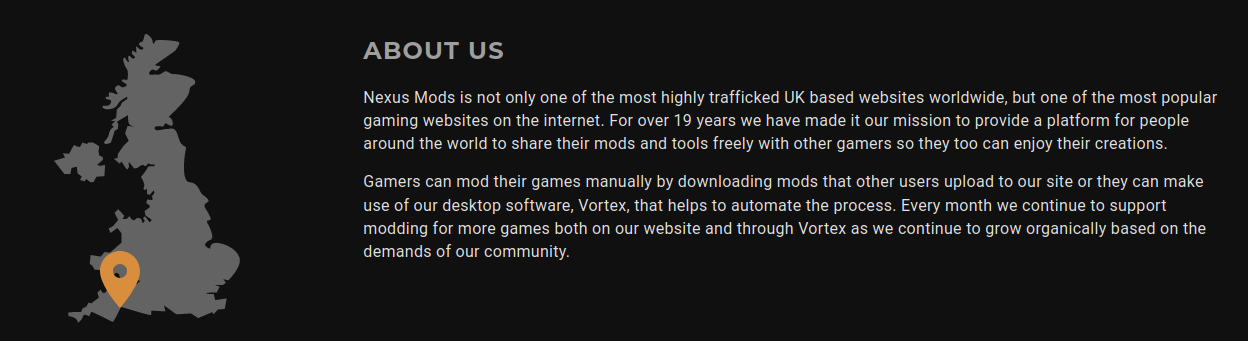
\includegraphics[width=16cm]{img/nexusmods_about_us.png}
    \caption{\textit{About Us} section of \textit{NexusMods}}
    \label{fig:nexusmods_about_us}
\end{center}
\end{figure}

As such, we can conclude that whois information did not provide us with significant information.

\subsection{DNS Dumpster}

Next, we shall use \url{dnsdumpster.com} to fetch DNS records and see if we get any IP addresses and IP ranges that would be of assistance to us.

\begin{figure}[H]
\begin{center}
    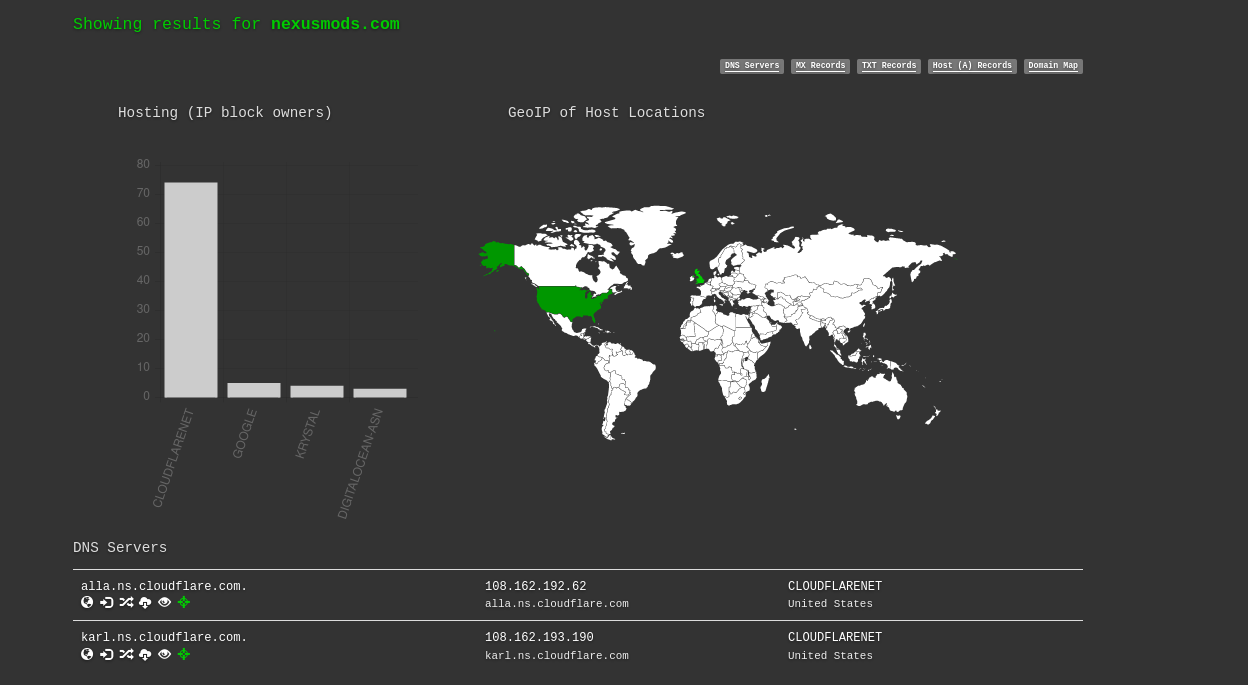
\includegraphics[width=16cm]{img/dumpster_start.png}
    \caption{Initial results on \textit{NexusMods} in \textit{DNS Dumpster}}
    \label{fig:dumpster_start}
\end{center}
\end{figure}

We can see some additional confirmation, some of IP addresses originate within UK, while a large portion is within US. This is most likely because \textit{NexusMods} uses Cloudflare as proxy and caching service (\autoref{fig:dumpster_start}). 

Additionally, we can see in these records as well, that the DNS servers the same ones that we have seen previously.

\begin{figure}[H]
\begin{center}
    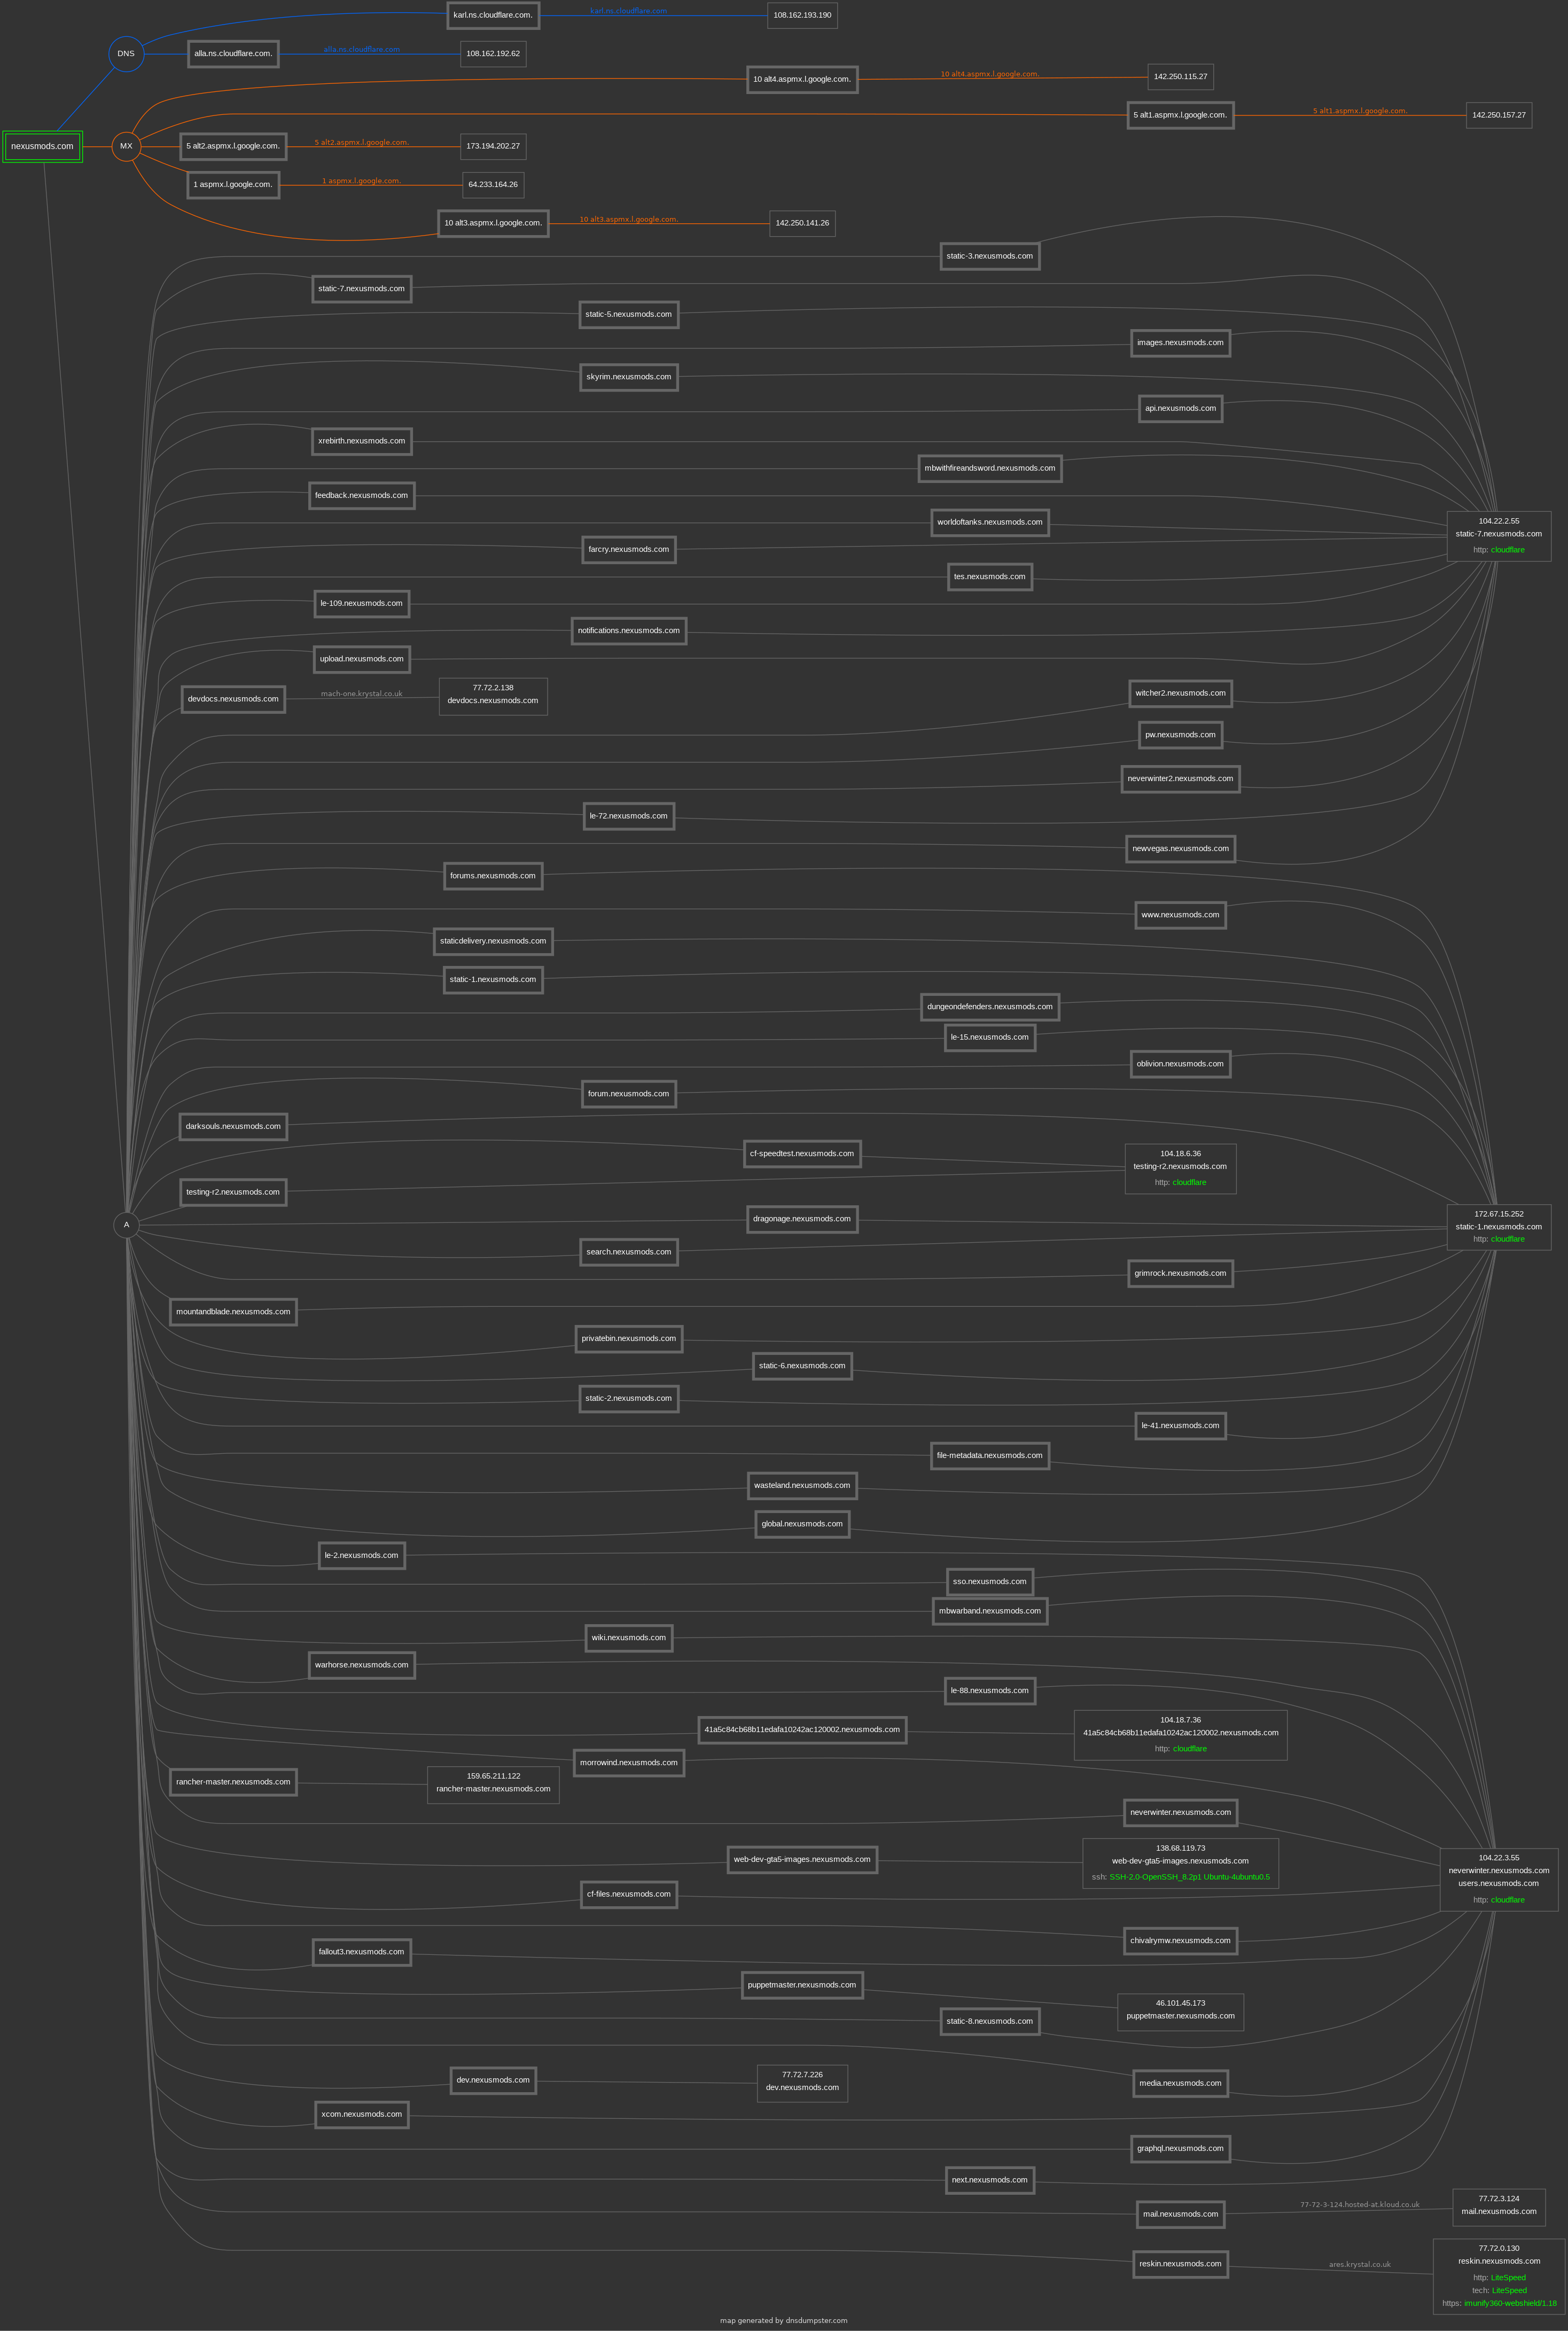
\includegraphics[width=16cm]{img/dns_map.png}
    \caption{DNS map of \textit{NexusMods} in \textit{DNS Dumpster}}
    \label{fig:dns_map}
\end{center}
\end{figure}

As we can see from DNS graph (\autoref{fig:dns_map}), it contains a large amount of DNS entries, and we will not be testing every single one. Let's look around and see if we can find any interesting subdomains, that might be of interest to us. 

\begin{figure}[H]
\begin{center}
    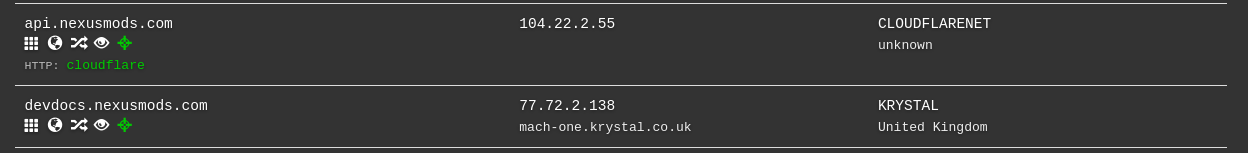
\includegraphics[width=16cm]{img/dns_api_docs.png}
    \caption{Interesting DNS entries for \textit{NexusMods} in \textit{DNS Dumpster}}
    \label{fig:dns_api_docs}
\end{center}
\end{figure}
    
We can see there's an endpoint for an API, as well as an endpoint for developer documentation (\autoref{fig:dns_api_docs}). Both these endpoints might have data that would be of interest to us, as such we shall see what is behind the IP addresses of \textit{104.22.2.55} and \textit{77.72.2.138}.

\subsection{\textit{nmap}}

\subsubsection{104.22.2.55}

A scan of \textit{104.22.2.55} provides us with some information (\autoref{fig:scan_1}).

\begin{figure}[H]
\begin{center}
    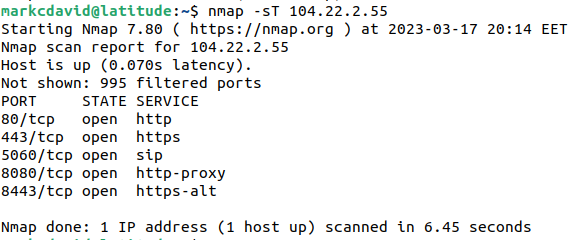
\includegraphics[width=16cm]{img/scan_1.png}
    \caption{\textit{nmap} scan of \textit{104.22.2.55}}
    \label{fig:scan_1}
\end{center}
\end{figure}
    

Trying to send a \textit{GET} request to the \textit{HTTP} port, we are met with \textit{403} response (\autoref{fig:scan_1_403}), which seems to be correct. From personal experience with the service, usage of the \textit{API} is reserved privillege for paying customers.

\begin{figure}[H]
\begin{center}
    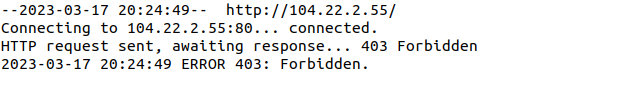
\includegraphics[width=16cm]{img/scan_1_403.png}
    \caption{\textit{GET} request to \textit{104.22.2.55}}
    \label{fig:scan_1_403}
\end{center}
\end{figure}

\subsubsection{77.72.2.138}

This server, as opposed to \textit{104.22.2.55} seems to be hosted in UK. \textit{NexusMods} are using services of \textit{Krystal} (\autoref{fig:krystal}), to provide documents for the developers.

\begin{figure}[H]
\begin{center}
    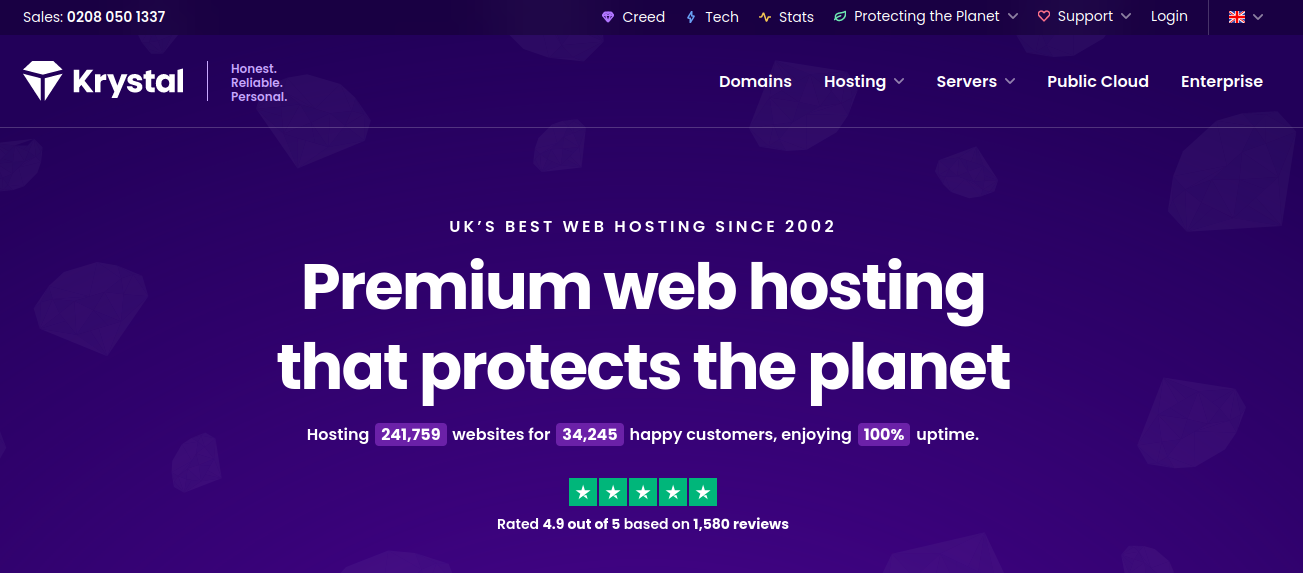
\includegraphics[width=16cm]{img/krystal.png}
    \caption{\textit{Krystal} homepage}
    \label{fig:krystal}
\end{center}
\end{figure}


Let's do a portscan for \textit{77.72.2.138} (\autoref{fig:scan_2}).

\begin{figure}[H]
\begin{center}
    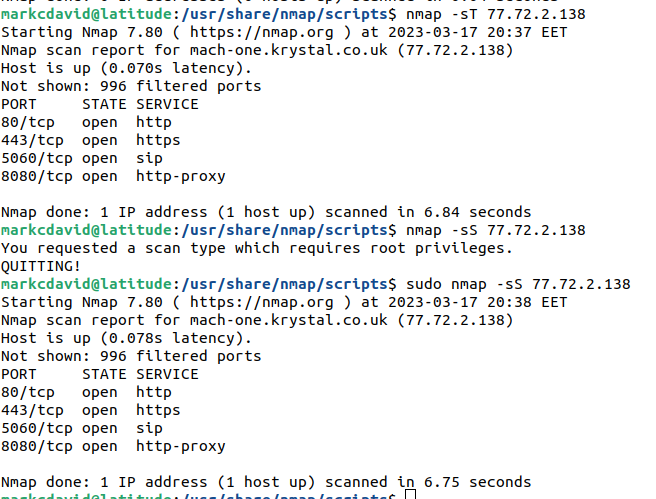
\includegraphics[width=16cm]{img/scan_2.png}
    \caption{\textit{nmap} scan of \textit{77.72.2.138}}
    \label{fig:scan_2}
\end{center}
\end{figure}

Similarly to \textit{104.22.2.55}, it provides a \textit{http} service, and if we try to send a \textit{GET} request we are met with timeouts, as the service does not answer our requests in any way (\autoref{fig:scan_2_timeout}).

\begin{figure}[H]
\begin{center}
    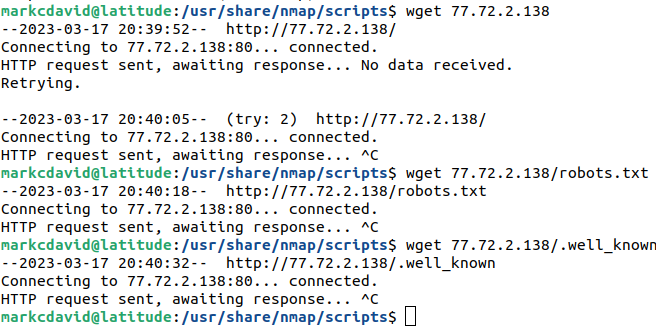
\includegraphics[width=16cm]{img/scan_2_timeout.png}
    \caption{\textit{GET} request to \textit{77.72.2.138}}
    \label{fig:scan_2_timeout}
\end{center}
\end{figure}

\VTDocumentEnd